\documentclass[11pt,letterpaper]{article}

\usepackage{showlabels}
\usepackage{fullpage}
\usepackage{pslatex}
%\usepackage{latexsym}
\usepackage[english]{babel}
\usepackage[utf8]{inputenc}
\usepackage{amsmath}
\usepackage{bm}
%\usepackage{tikz}
\usepackage{xcolor}
\usepackage{url}
%\usepackage[colorinlistoftodos]{todonotes}
\usepackage{rotating}
\usepackage{natbib}
\usepackage{amssymb}
\usepackage{lingmacros}


\usepackage{natbib}
\bibliographystyle{unsrtnat}

%\usepackage{latexsym}
\usepackage[english]{babel}
\usepackage[utf8]{inputenc}
\usepackage{bm}
\usepackage{graphicx}
%\usepackage{tikz}
\usepackage{xcolor}
\usepackage{url}
%\usepackage[colorinlistoftodos]{todonotes}
\usepackage{rotating}
\usepackage{multirow}


%\usepackage{linguex}
%\usepackage{lingmacros}


\usepackage{hyperref}

\usepackage{tikz-dependency}
\usepackage{changepage}
\usepackage{longtable}


\newcommand{\R}[0]{\mathbb{R}}
\newcommand{\Prob}[0]{\mathbb{P}}
\newcommand{\Ff}[0]{\mathcal{F}}

\usepackage{multirow}

\newcommand{\soft}[1]{}
\newcommand{\nopreview}[1]{}
\newcommand\comment[1]{{\color{red}#1}}
\newcommand\mhahn[1]{{\color{red}(#1)}}
\newcommand\note[1]{{\color{red}(#1)}}
\newcommand\jd[1]{{\color{red}(#1)}}
\newcommand\rljf[1]{{\color{red}(#1)}}
\newcommand{\key}[1]{\textbf{#1}}

\DeclareMathOperator*{\argmax}{arg\,max}
\DeclareMathOperator*{\argmin}{arg\,min}
\DeclareMathOperator{\E}{\mathop{\mathbb{E}}}



\usepackage{amsthm}

\newcommand{\thetad}[0]{{\theta_d}}
\newcommand{\thetal}[0]{{\theta_{LM}}}

\newcounter{theorem}
\newtheorem{proposition}[theorem]{Proposition}
\newtheorem{thm}[theorem]{Theorem}
\newtheorem{corollary}[theorem]{Corollary}
\newtheorem{question}[theorem]{Question}
\newtheorem{example}[theorem]{Example}
\newtheorem{defin}[theorem]{Definition}
\newtheorem{definition}[theorem]{Definition}
\newtheorem{lemma}[theorem]{Lemma}


%\usepackage{linguex}
%\newcommand{\key}[1]{\textbf{#1}}



\renewcommand{\thefigure}{S\arabic{figure}}
\renewcommand{\thetable}{S\arabic{table}}
\renewcommand{\thesection}{S\arabic{section}}

\newcommand{\utterance}{\mathcal{U}}
\newcommand{\tree}{\mathcal{T}}



\usepackage{siunitx}



\usepackage{longtable}



\frenchspacing
%\def\baselinestretch{0.975}

%\emnlpfinalcopy
%\def\emnlppaperid{496}

\title{Morpheme Ordering across Languages reflects optimization for memory efficiency / information locality}

\begin{document}

\maketitle

\begin{abstract}
    The order of morphemes in a word shows well-documented tendencies across languages.
    These have been explained in terms of notions such as semantic scope and relevance in prior work.
A recent theory (CITE) argues that word and morpheme order in language optimizes a tradeoff between Memory and surprisal, and provided initial evidence from twoi languages that morpheme order can partly be explained by optimization for this treadeoff.
    %Efficient memory--surprisal tradeoffs are achieved by orders that display information locality, whereby elements that have high mutual information are closer together.
    In this work, we test this idea more extensively using data from four additional agglutinative languages with significant amounts of morphology.
    
%    In this work, we examine corpus data from four languages to show that optimizing for tradeoff efficiency mostly predicts morpheme order in verb and noun morphology.
    
\end{abstract}



\section{Introduction}

Across languages, words are composed of morphemes, commonly defined as the smallest meaning-bearing units of language.
Morphemes can take different shapes.
In many cases, words can be segmented into a sequence of morphemes, as in the English word runners (root run-, derivation -er-, plural -s).
The order of morphemes within a word follows well-documented cross-linguistic tendencies, for instance, plural markers tend to be closer to noun stems than case markers \citep[112]{greenberg1963universals}.
These tendencies have been explained in terms of the relative scope of different morphemes  \citep{givon1971historical,venneman1973explanation,baker1985the,rice2000morpheme} and the strength of their semantic association with the root \citep{bybee-morphology-1985}.
%One family of explanations holds that those affixes are closest to the root that are most relevant to the root \citep{bybee-morphology-1985}.
%Other explanations suggest that morphemes are ordered based on (TODO CITE).

A recent theory proposes a cognitive explanation for these tendencies, arguing that ordering universals in language can be understood as arising from optimization of processing effort under memory limitations \citep{Hahn2020modeling}.
Formally, they introduced the notion of a memory-surprisal tradeoff: Depending on how many memory resources a comprehender invests, they can achieve different levels of surprisal.
(CITE) hypothesize that order of words and morphemes in language optimizes this tradeoff.
Optimizing the memory-surprisal tradeoff amounts to putting elements together when they predict each other strongly, as measured by mutual information.
In a case study, CITE apply this to morpheme ordering in Japanese and Sesotho, finding that optimization could partly reproduce morpheme ordering in these languages.
They also suggested that mutual information formalizes previous notions of strength of semantic association, such as \cite{bybee-morphology-1985}'s notion of \textit{relevance}.


In this work, we examine this theory on a broader basis by considering data from four additional languages.
We focus on languages where words tend to have multiple morphemes and these are mostly realized separately. Such languages are referred to as agglutinative (Greenberg 1954).
We obtained data from four languages (Korean, Turkish, Hungarian, Finnish).
Whereas \cite{Hahn2020modeling} only considered verb inflection, we also consider noun inflection across three languages.


%Greenberg 1963:  "the expression of number almost always comes between the noun base and the expression of case" (Greenberg 1963:112)

%Scope, Syntax, History
%Another family of explanations holds that morpheme ordering is to be explained diachronically, and that morpheme order reflects the order of independent words in earlier stages of a language.
%- Relevance, Proximity Principle, Iconicity




%Bybee on explanation:
%- regarding the historical explanation (Givon 1971, Vennemann 1973):
%Morphology is not always fossilizes syntax (Bybee and Brewer 1980, Bybee 1985 p. 39--40)


\section{Morpheme Ordering and Ordering Universals}

In this section, we introduce some general crosslinguistic tendencies in morpheme ordering, before discussing data from the six languages in Section XX.

\paragraph{Nouns}
Nouns commonly mark number and case.
For nouns, \citep[112]{greenberg1963universals} Universal 39 states that number affixes are closer to the stem than case affixes, if they appear on the same side.
In some languages, possession is also marked on the noun.

\paragraph{Verbs}
Verbs commonly mark a larger number of inflection categories.
Based on data from several dozens of languages, \citep{bybee-morphology-1985} proposes the following ordering of verb affixes:
\begin{quote}
\begin{tabular}{llllllllllllllllllllllllll}
verb stem & valence & voice & aspect & tense& mood & subject agreement
\end{tabular}
\end{quote}
\textit{Valence} affixes change the number of arguments; for instance, causatives add an argument (TODO example).
\textit{Voice} describes the distinction between active and passive.
\textit{Aspect} describes how an event unfolds over time, such as the English progressive -ing indicating that an action  is still ongoing.
\textit{Tense} describes where an event is located in time (e.g. past or future).
\textit{Mood} TODO \textit{Modality} TODO
\textit{Subject person and number} mark categories of the subject, such as English third-person -s.

While these are particularly common types of affixes, there are further types.
Examples are polarity (negation), evidential (based on what evidence a speaker makes an assertion), and formality.


We focus on inflection, except in those cases where derivational affixes are clearly marked in available data.
Inflectional suffixes are generally outside of derivational affixes


\section{Background: Memory--Surprisal Tradeoff and Information Locality}

\citet{Hahn2020modeling} introduced the Memory--Surprisal Tradoff as a cognitive account of the order of words and morphemes in human language, based on a formalization of memory efficiency in incremental processing.

The memory-surprisal tradeoff links information-theoretic models of memory limitations with surprisal theory.
Surprisal theory \citep{hale2001probabilistic, levy2008expectation} states that the processing effort on a word $w_t$ in context $w_1 ... w_{t-1}$ is proportional to its surprisal
     \begin{equation}   \label{eq:true-surp}
    \text{Difficulty} \propto -\log P(w_t | w_1\dots w_{t-1}).
\end{equation}
Surprisal as estimated by corpus-based methods is a successful predictor of reading time on naturalistic text \citep{smith2013effect,goodkind-predictive-2018,frank2019interaction,aurnhammer2019evaluating,wilcox2020predictive}.
This effect can be explained in terms of mechanisms such as preactivation and integration~\citep{kuperberg2016we}.
However, due to limitations in human memory, human expectations in reality do not reflect the true context $w_1\dots w_{t-1}$, but some memory representation $m_t$:
\begin{equation}   \label{eq:lossy-surp}
    \text{Difficulty} \propto -\log P(w_t | m_t).
\end{equation}
\citet{Hahn2020modeling} note that there is a tradeoff between average surprisal and memory capacity:
The more information a listener stores in $m_t$, the lower their surprisal will be on average.
This is because higher precision of memory leads to more precise expectations, which will achiever lower surprisal on average.
More formally, given a function $M$ encoding contexts $w_1\dots w_{t-1}$ into memory representations $m_t$, there is a tradeoff between, on the one hand, the average surprisal $S_M$, obtained by averaging $-\log P(w_t | m_t)$ across the words in a text, and the memory capacity $H_M$, formalized as the average number of bits required to encode $m_t$.


\citet{Hahn2020modeling} prove a theorem that provides a method of estimating the memory-surprisal tradeoff from corpus data.
This theorem is based on \key{mutual information}, which quantifies the amount of statistical association between two random variables.
If $X, Z, Y$ are random variables, then the mutual information of $X$ and $Y$, conditioned on $Z$, is defined to be:
\begin{align}
\label{eq:mi}
    \operatorname{I}[X:Y|Z] &\equiv \sum_{x,y,z} P(x,y,z) \log \frac{P(x,y|z)}{P(x|z)P(y|z)}. % \text{ bits} \\
    %\nonumber
    %&= \operatorname{H}[X|Z] - \operatorname{H}[X|Y,Z] \\
    %\nonumber
    %&= \operatorname{H}[Y|Z] - \operatorname{H}[Y|X,Z].
\end{align}
The key quantity derived from this is the mutual information between elements (such as morphemes) that are some distance $t$, conditioned on the intervening elements:
\begin{equation*}
    I_t \equiv \operatorname{I}[w_t : w_0 | w_1, \dots, w_{t-1}].
\end{equation*}
Based on this notion, \citet{Hahn2020modeling}  prove the following bound on the memory-surprisal tradeoff ($S_\infty$ is the average surprisal that would be achieved with perfectly veridical memory representations):
\begin{thm}\label{prop:suboptimal}(Information locality bound, \citet{Hahn2020modeling})
For any positive integer $T$, let $M$ be a memory encoding function such that
\begin{equation}
\label{eq:memory-bound}
H_M \le \sum_{t=1}^T t I_t.
\end{equation}
Then we have a lower bound on the average surprisal under the memory encoding function $M$:
\begin{equation}
\label{eq:surprisal-bound}
S_M \ge S_\infty + \sum_{t=T+1}^\infty I_t.
\end{equation}
\end{thm}


A key consequence of this theorem is that it implies information locality:
Orderings optimize this tradeoff when elements with high mutual information are closer together.
A similar notion of information locality was previous derived by \citet{futrell2020lossy} for a specific family of memory representations $M$.
Information locality has had success as a predictor of word order \citep{futrell2019information}, in particular for universals of the order inside noun phrases \citep{culbertson2020from,hahn-information-theoretic-2018,DBLP:conf/acl/FutrellDS20}.

\citet{Hahn2020modeling} argue that information locality derives a range of locality principles proposed in the linguistic literature, including \cite{bybee-morphology-1985}'s idea that morphemes are closer together when they are more relevant to each other.
\mhahn{say more about relevance}

\section{Methods}

\subsection{Data} % TODO: Becky
% why agglutinative?
We considered:

- UD data for Japanese, Korean, Turkish, Hungarian, Finnish

- CHILDES data for Sesotho

The Sesotho and Japanese data was previously used by CITE; we reanalyze these data here in a way consistent across all six languages.


\subsection{Nouns}

\paragraph{Turkish Nouns}
\begin{enumerate}
    \item Number
    \item Possessor number and possessor person
    \item Case 
\end{enumerate}

\paragraph{Hungarian Nouns}
\url{https://cl.lingfil.uu.se/~bea/publ/megyesi-hungarian.pdf}
\begin{enumerate}
    \item Number
    \item Possessor person
    \item Possessor number
    \item Case 
\end{enumerate}

\paragraph{Finnish Nouns}
\begin{enumerate}
    \item Derivation
    \item Number
    \item Case 
    \item Possessor person and possessor number
\end{enumerate}

\subsection{Verbs}

\paragraph{Hungarian Verbs}
\begin{enumerate}
    \item Voice
    \item Tense 
    \item Mood
    \item Definiteness, person, and number
\end{enumerate}

\paragraph{Turkish Verbs}
\begin{enumerate}
    \item Voice
    \item Negation / polarity
    \item Aspect
    \item Evidential 
    \item Tense 
    \item Mood 
    \item Person and Number
    \item Formality
\end{enumerate}

\paragraph{Finnish Verbs}
\begin{enumerate}
    \item Voice
    \item Tense 
    \item Mood 
    \item Person and number
    \item Clitic
\end{enumerate}

\paragraph{Sesotho Verbs}
We describe Sesotho verb affixes following \cite{Hahn2020modeling}.
who described these based on \citep{doke1967textbook, guma1971outline, demuth1992acquisition}

\begin{enumerate}
    \item Subject agreement: This morpheme encodes agreement with the subject, for person, number, and noun class (the latter only in the 3rd person) \cite[\textsection 395]{doke1967textbook}.
            The annotation provided by \cite{demuth1992acquisition} distinguishes between ordinary subject agreement prefixes and agreement prefixes used in relative clauses; we distinguish these morpheme types here.

    \item Negation \citep[\textsection 429]{doke1967textbook}

    \item Tense/aspect marker   \citep[\textsection 400--424]{doke1967textbook}

    \item Object agreement or reflexive marker \citep[\textsection 459]{doke1967textbook}.
    Similar to subject agreement, object agreement denotes person, number, and noun class features of the object.
\end{enumerate}
We identified the following suffixes:

\begin{enumerate}
\item Semantic derivation: reversive (e.g., `do' $\rightarrow$ `undo')
\item Valence: (e.g., causative, neuter/stative, applicative, and reciprocal)
    \item Voice: passive
    \item Tense
    \item Mood
    \item Interrogative and relative markers
\end{enumerate}



\paragraph{Japanese Verbs}
We describe Japanese verb suffixes following \citep{Hahn2020modeling}, who described these based on \citep{kaiser2013japanese,hasegawa2014japanese}.

\begin{enumerate}
\item \textit{suru}: obligatory suffix after Sino-Japanese words when they are used as verbs
\item Valence: causative (-\textit{ase}-)
\item Voice and Mood: passive (-\textit{are}-, -\textit{rare}-) and potential (-\textit{e}-, -\textit{are}-, -\textit{rare}-)
\item Politeness (-\textit{mas}-)
\item Mood: desiderative (-\textit{ta}-)
\item Negation (-\textit{n}-)
\item Tense, Aspect, Mood, and Finiteness: past (-\textit{ta}), future/hortative (-\textit{yoo}) \citep[229]{kaiser2013japanese}, nonfiniteness (-\textit{te})
\end{enumerate}



\paragraph{Korean Verbs}

We then considered morphemes occurring at least 50 times:

\citep{yeon2010korean}

\begin{enumerate}
    \item Root (Valency is not separated in the dataset)
    \item Derivation:
    
    ha (from hada, \citep[4.1.2]{yeon2010korean}), i (predicative, \citep[4.1.4]{yeon2010korean})
    
    \item Honorific -s- \citep[4.3.2, 4.4.1]{yeon2010korean}
    \item Tense/Aspect: -ess- for past \citep[4.5.1.1]{yeon2010korean}, -essess- for remote past \citep[4.5.1.2]{yeon2010korean}, -keyss- for future \citep[4.5.2.1]{yeon2010korean}
    \item Formality -p- \citep[4.3.2]{yeon2010korean}
    \item Mood 1:
    
    -n-
    
    -ni- \citep[4.3.2]{yeon2010korean}
    
    -ri-
    
    -deon-
    
    \item `Pragmatic Mood'
    
    -da- \citep[4.3.2]{yeon2010korean}
    
    -ra- 
    
    Interrogative -ka, -lkka, -nya
    
    -ji \citep[4.2.2-3]{yeon2010korean}
    
    -eo (informal)
    
    -sida \citep[4.3.2]{yeon2010korean}
    
    ....
    
    \item Polite -yo
    \item Conjunctive endings
    
    -go
    
    -seo
    
    and others
    
\end{enumerate}

TODO 

- Yeon 4.4.2.2 kkeo object honorific % 꺼

%\ex.\ag. oa di rek a \\
%\textsc{subject.agreement} \textsc{object.agreement} buy \textsc{indicative} \\
%`(he) is buying (it)'  \citep{demuth1992acquisition} \label{ex:oadireka}
%\bg. o pheh el a \\
%\textsc{subject.agreement} cook \textsc{applicative} \textsc{indicative} \\
%`(he) cooks (food) for (him)'  \citep{demuth1992acquisition}
%\label{ex:ophehela}


For SI Appendix:

Here, we explain how our segmentation corresponds to the speech style system described by \citep[4.3.2]{yeon2010korean}

\begin{tabular}{l|lllllll}
            & Statement & Question  & Command    & Proposal    \\ \hline
Formal      &  -p-ni-da & -p-ni-kka & -si-p-siyo & -si-p-sida \\
Polite      &  \multicolumn{4}{c}{-a/eo/yo} \\
Semi-Formal &  -o/so    &           & -o         & -p-sida \\
Familiar    &  -ne      & -na/neunja & -je       & -se     \\
Intimate    &  \multicolumn{4}{c}{-a/eo} \\
Plain       &  -da      &  -(neu)nya & -ra       & -sa \\
\end{tabular}

Examples:
\begin{tabular}{llllllllll}
1    & 3 & 4     & 5   & 6  & 7 & 8 \\
bara & sy & eots & eum & ni & da  & &  `wished'\\
wish & Honorific & Past & Formal & Indicative & Indicative \\
bara& & gess &  & &  eo & yo  &  `will wish' \\
wish  & &  Assertive && & informal & polite \\
\end{tabular}

%https://en.wiktionary.org/wiki/%EB%B0%94%EB%9D%BC%EB%8B%A4

\section{Results}

\begin{figure}
    \centering
    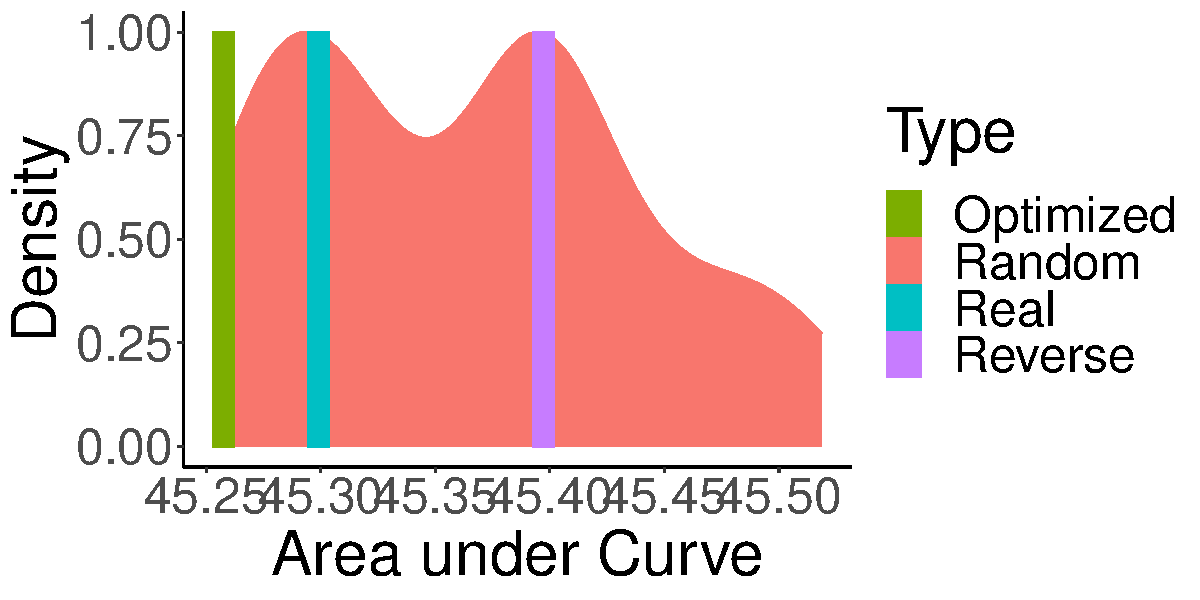
\includegraphics[width=0.4\textwidth]{figures/Hungarian-suffixes-byMorphemes-auc-hist-heldout-Coarse-FineSurprisal-optimized.pdf}
    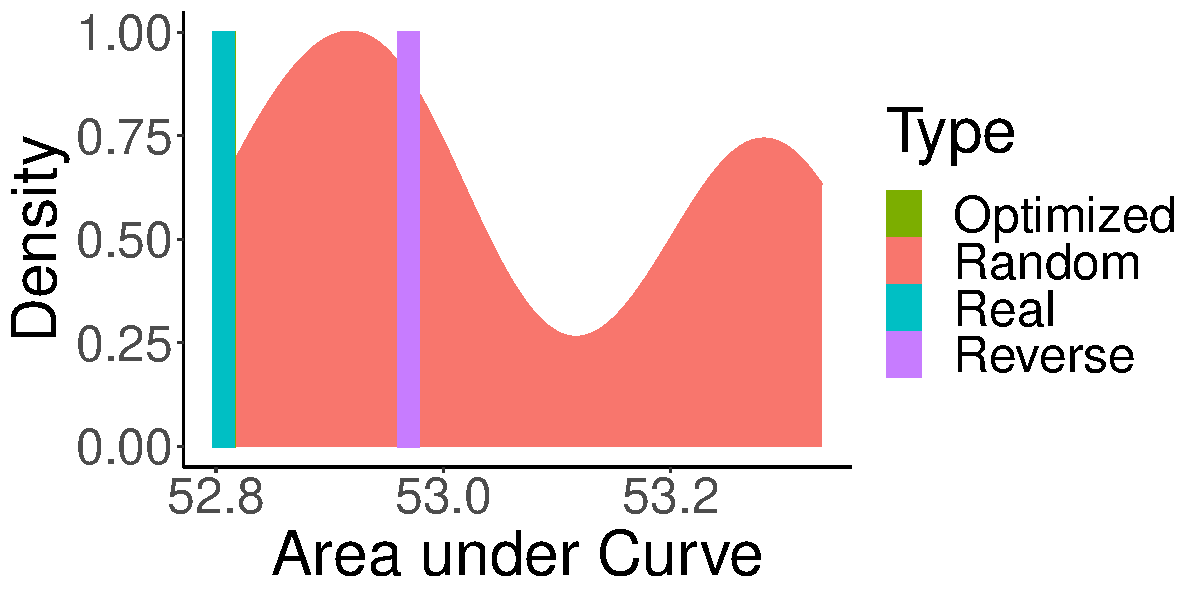
\includegraphics[width=0.4\textwidth]{figures/Hungarian-suffixes-byMorphemes-auc-hist-heldout-Nouns-Coarse-FineSurprisal-optimized.pdf}
    
    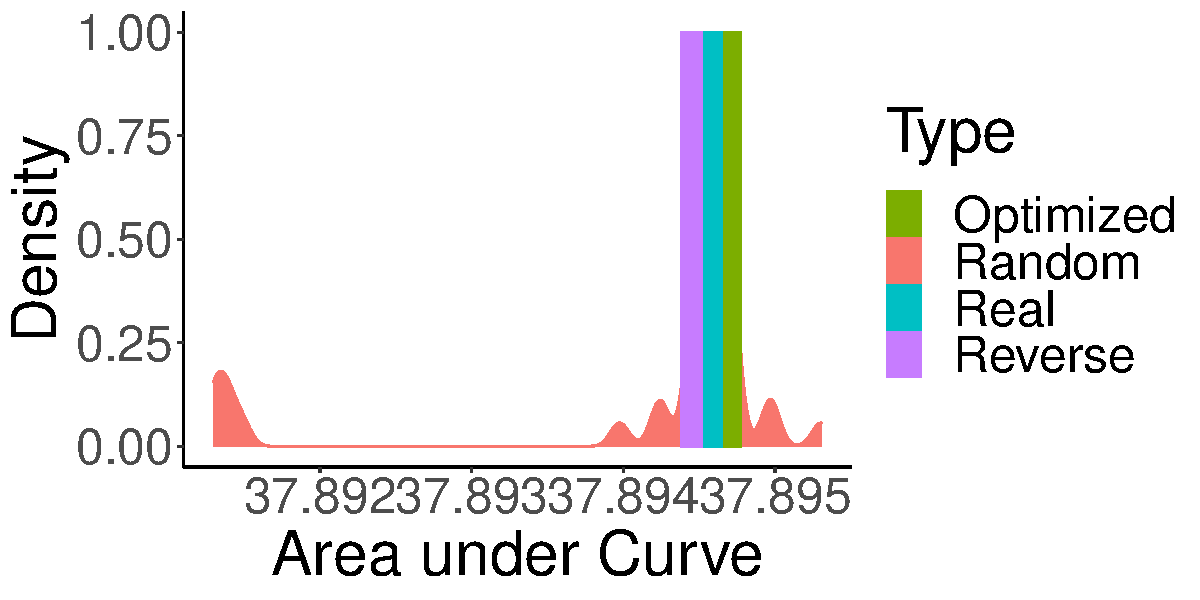
\includegraphics[width=0.4\textwidth]{figures/Turkish-suffixes-byMorphemes-auc-hist-heldout-Coarse-FineSurprisal-optimized.pdf}
    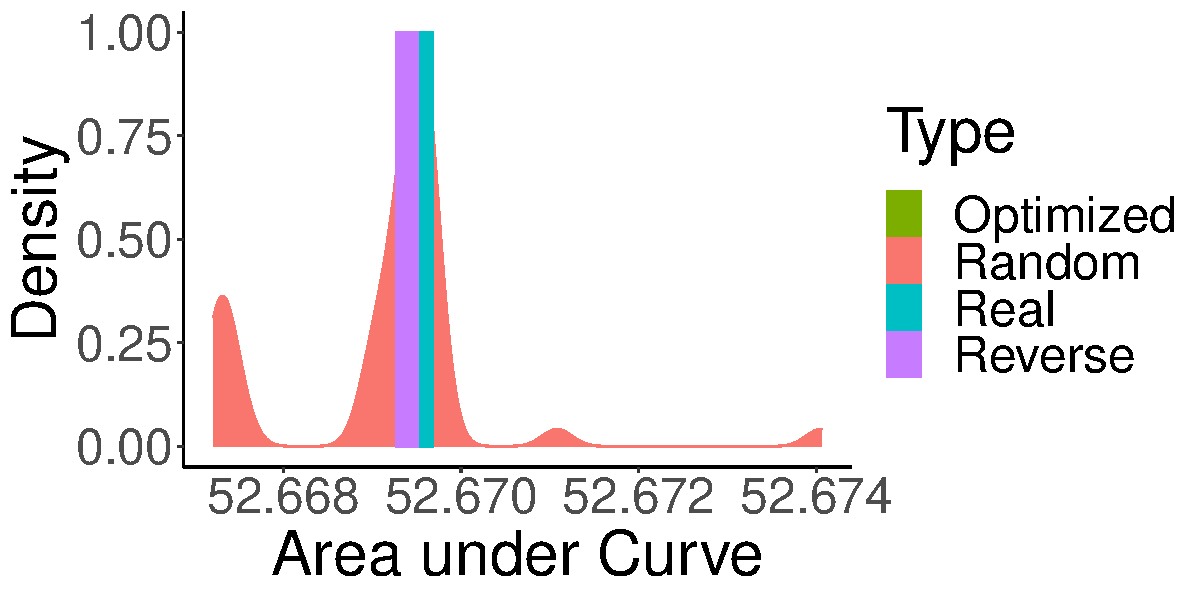
\includegraphics[width=0.4\textwidth]{figures/Turkish-suffixes-byMorphemes-auc-hist-heldout-Nouns-Coarse-FineSurprisal-optimized.pdf}
    \caption{Caption}
    \label{fig:my_label}
\end{figure}

\section{Discussion}

We have examined morpheme order in nouns and verbs in six languages, testing the recently propiosed Efficient Tradeoff Hypothesis \citep{hahn2020modeling} as an explanatory account of morpheme ordering.
We compared actual morpheme orderings to other possible orderings and to orderings optimized for efficiency of the memory-surprisal tradeoff.
In most cases, we found that the real ordering provided almost more efficient tradeoffs than most alternative orderings.
More importantly, we found that the real orderings match the optimal orderings in many respects.
Ordering forms found in a corpus according according to real or optimized orderings yields the same orders in XXX of cases.
In some cases, particlarly for noun inflection, match between real and optimized orderings is perfect.

\subsection{Relation to previous accounts}

%\subsubsection{Semantic Scope; Syntactic Structure; Historical Development}

In this section, we discuss the linguistic literature on morpheme ordering.

\paragraph{Meaning and Scope}


Besides Bybee's account in terms of relevance, there are also accounts focusing on semantic scope \citep{rice2000morpheme}.

Also noted scope: \citep{baker1988incorporation,foley1984functional,chierchia1990meaning,valin1992a}



\paragraph{Morpheme Order and Word Order}
It has long been observed that the order of morphemes often parallels the order of independent words of corresponding meanings \citep{givon1971historical,venneman1973explanation,baker1985the}.
It has been argued that the order of morphemes reflects the order of formerly independent elements that have been fossilized into bound morphemes \citet{givon1971historical,venneman1973explanation}.
As the memory-surprisal tradeoff is optimized by word order, this is compatible with our results:
To the extent that morpheme order does reflect fossilized word order, morpheme order should continue to reflect optimization for the tradeoff.

On the other hand, \citet{bybee-morphology-1985} points out that there are historically documented cases where morpheme ordering has been restructured in ways that do not reflect former independent words, but respect the universal tendencies proposed by her (see also \citet{mithun2000the, haspelmath1993the, mithun1995affixation}; \citet[Section 15]{rice2000morpheme}).


\paragraph{Levels of Linguistic Description}
Besides the explanation of broad typological tendencies, which we are interested in here, the linguistic literature has also debated at which level of linguistic representation morpheme ordering should be described, proposing accounts located at different levels such as the syntax-phonology interface \citep{baker1985the} and an autonomous layer of morphological description \citep{hyman2003suffix}.
TODO also template vs scope vs...
We do not see the memory--surprisal tradeoff as competing with or contradicting these studies.
Rather, it specifies tendencies for ordering that could be implemented at different levels of linguistic description.




%One family of explanations holds that those affixes are closest to the root that are most relevant to the root \citep{bybee-morphology-1985}.
%Other explanations suggest that morphemes are ordered based on (TODO CITE).
%The most straightforwardly related account is that of Bybee (1985) Semantic relevance
%CARP template in Bantu
%Explanations for the orders
%A related, though different, account is in terms of semantic scope \cite{rice2000morpheme}.
%The scope hypothesis is attractive for some morphemes.
%For instance, 
%\cite{baker1985the} proposed the Mirror Principle, stating that the order of morphemes reflects ...
%This can be related to the scope-based explanation to the extent that syntactic structure and word order reflect scope.
%\cite{muysken1981quechua}
%\cite{mccarthy2008generalized} phonology
%\cite{hyman2003suffix}
%\cite{kanu2009suffix} morphotactics, not semantic scope


%\subsection{Relevance; Proximity; Iconicity}

%The relation  between mutual information and relevance

\subsection{Beyond Agglutionation}

Our study focused on agglutinatioon, where a word carries multiple clearly separated morphemes with distinct functions.
There are other types of morphological processes that deserve study.

While we have focused on the relative distance from the root, we have not touched on the question of why a morpheme is realized as a prefix or a suffix in a given language.
There are well-known correlations between suffixing or prefixing preference and word order \citep{greenberg1963universals}.

- infixation

Vowel change, productive in many languages and fossilized in English (swim $\rightarrow$ swam).

non-concatenative morphology (in Arabic, k-t-b `to write' forms katab- `wrote'. -aktub `write/be writing', -kutib- `was written').

\subsection{Limitations}

- genre of data: written



\section{Conclusion}

\bibliography{literature}
\bibliographystyle{natbib}

\end{document}






